\section{Esimerkki liitteestä\label{LiiteA}}

Liitteet eivät ole opinnäytteen kannalta välttämättömiä ja 
opinnäytteen tekijän on 
kirjoittamaan ryhtyessään hyvä ajatella pärjäävänsä ilman liitteitä.
Kokemattomat kirjoittajat, jotka ovat huolissaan
tekstiosan pituudesta, paisuttavat turhan 
helposti liitteitä pitääkseen tekstiosan pituuden annetuissa rajoissa.
Tällä tavalla ei synny hyvää opinnäytettä.   

Liite on itsenäinen kokonaisuus, vaikka se täydentääkin tekstiosaa.
Liite ei siten ole pelkkä listaus, kuva tai taulukko, vaan 
liitteessä selitetään aina sisällön laatu ja tarkoitus. 

Liitteeseen voi laittaa esimerkiksi listauksia. Alla on 
listausesimerkki tämän liitteen luomisesta. 

%% Verbatim-ympäristö ei muotoile tai tavuta tekstiä. Fontti on monospace.
%% Verbatim-ympäristön sisällä annettuja komentoja ei LaTeX käsittele. 
%% Vasta \end{verbatim}-komennon jälkeen jatketaan käsittelyä.
\begin{verbatim}
	\clearpage
	\appendix
	\addcontentsline{toc}{section}{Liite A}
	\section*{Liite A}
	...
	\thispagestyle{empty}
	...
	tekstiä
	...
	\clearpage
\end{verbatim}

Kaavojen numerointi muodostaa liitteissä oman kokonaisuutensa:
\begin{align}
d \wedge A &= F, \label{liitekaava1}\\
d \wedge F &= 0. \label{liitekaava2}
\end{align}


\clearpage
\section{Toinen esimerkki liitteestä\label{LiiteB}}

%% Liitteiden kaavat, taulukot ja kuvat numeroidaan omana kokonaisuutenaan

Liitteissä voi myös olla kuvia, jotka
eivät sovi leipätekstin joukkoon:
%% Ympäristön figure parametrit htb pakottavat
%% kuvan tähän, eikä LaTeX yritä siirrellä niitä
%% hyväksi katsomaansa paikkaan. 
%% Ympäristöä center voi käyttää \centering-
%% komennon sijaan
%%
%\begin{figure*}[htb]
%\centering
%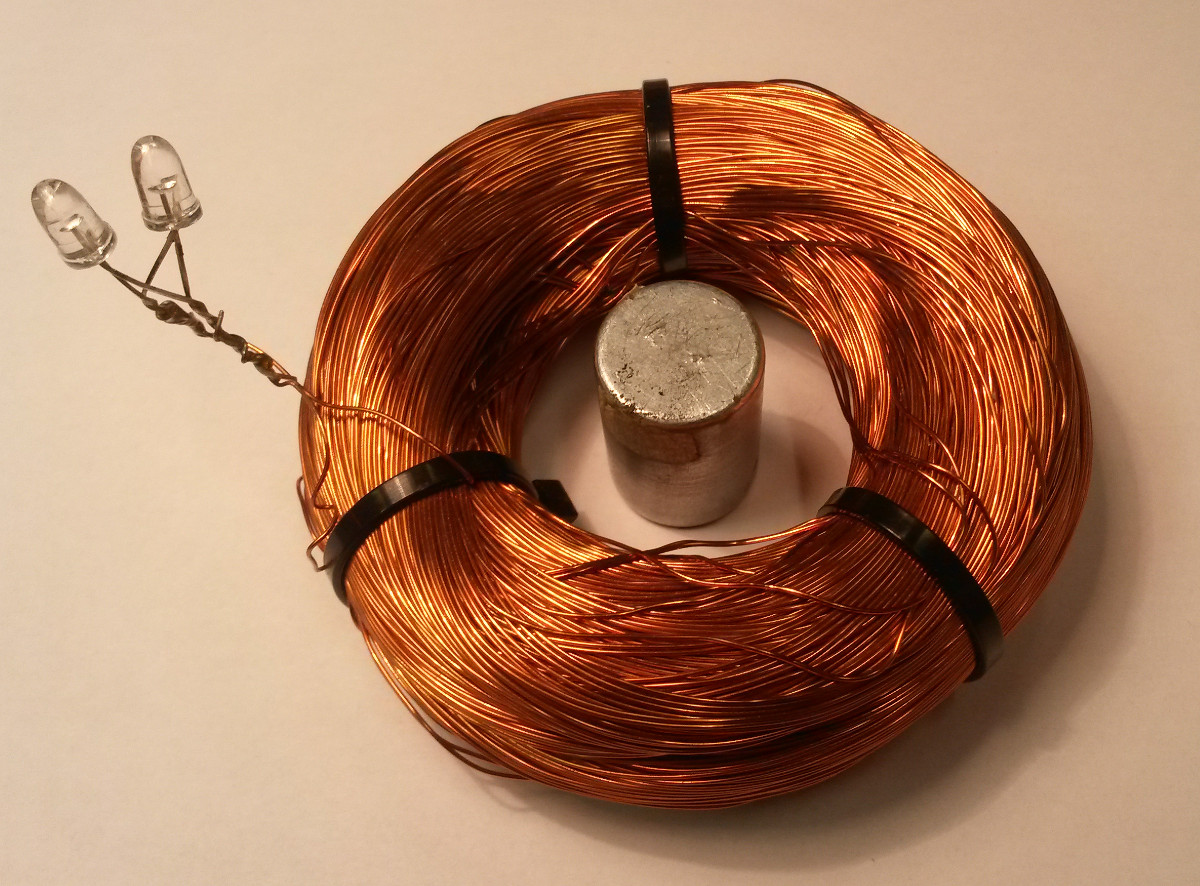
\includegraphics[height=8cm]{figures/ledspole.jpg}
%\caption{Kuvateksti, jossa on liitteen numerointi}
%\label{liitekuva}
%\end{figure*}
%%
Liitteiden taulukoiden numerointi on kuvien ja kaavojen kaltainen:
\begin{table}[htb]
\caption{Taulukon kuvateksti.}
\label{liitetaulukko}
\centering
\begin{tabular}{|lp{0.5\linewidth}|}
\hline
9.00--9.55  & Käytettävyystestauksen tiedotustilaisuus (osanottajat
ovat saaneet sähköpostitse valmistautumistehtävät, joten tiedotustilaisuus
voidaan pitää lyhyenä).\\
9.55--10.00 & Testausalueelle siirtyminen \\
\hline
\end{tabular}
\end{table}
Kaavojen numerointi muodostaa liitteissä oman kokonaisuutensa:
\begin{align}
T_{ik} &= -p g_{ik} + w u_i u_k + \tau_{ik},  \label{liitekaava3} \\
n_i    &= n u_i + v_i.                      \label{liitekaava4}
\end{align}

\clearpage
\section{Matemaattisten lauseiden todistukset\label{LiiteC}}
Systeemianalyysin töissä matemaattisten lauseiden todistukset laitetaan yleensä liitteiksi. Leipätekstissä lauseen yhteydessä todistuksen todetaan löytyyvän liitteestä XX. Tämä ei koske matematiikan töitä, joissa lauseiden todistukset voivat olla merkittävä osa varsinaista työtä!
\begin{maaritelma}
Tässä määritellään $1=1$.
\end{maaritelma}

\begin{lause}[Roposen lause]\label{thrm:roponen}
Lukiomatematiikassa kolmannen asteen yhtälöillä on aina vähintään yksi kokonaislukuratkaisu välillä $[-3,3]$.
\end{lause}
\begin{proof}
Jätetään harjoitustehtäväksi.
\end{proof}

\begin{huomautus}
Lause \ref{thrm:roponen} saattaa olla väärin.
\end{huomautus}

Tiedoston opinnaytepohja.tex alusta löytyy myös muita teoreema- ym. tyylejä sekä suomeksi että englanniksi, joten katso löytyykö sieltä käyttöösi sopiva. Voit myös määritellä itse lisää.